\documentclass[12pt, a4paper]{article}
\title{Chapter 1}
\author{Maciej Harbuz}
\usepackage{amssymb}
\usepackage{amsmath}
\usepackage{tikz} 
\usepackage{import}
\usepackage{float}
\usetikzlibrary{automata, positioning, arrows}
\includeonly{chapter01-exercises-113-115.tex}
\tikzset{
    ->, % makes the edges directed
    every state/.style={thick, fill=gray!15}, % sets the properties for each ’state’ node
    node distance=2.5cm, % specifies the minimum distance between two nodes. Change if necessary.
    initial text=$ $, % sets the text that appears on the start arrow
    >=stealth, % makes the arrow heads bold
}

\begin{document}

\maketitle

\section{Exercises}
%\subfile{chapter00-exercises}
%\import{./}{chapter01-exercises-101-106.tex}
%\import{./}{chapter01-exercises-107-112.tex}
%\import{./}{chapter01-exercises-113-115    .tex}
\begin{enumerate}

    \item[1.1]
          The following are the state diagrams of two DFAs, $M_1$ and $M_2$. Answer the following questions about each of these machines.

          \begin{figure}[H]
              \centering
              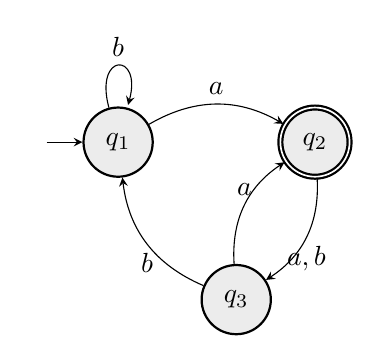
\begin{tikzpicture}
                  \node[state, initial] (q1) {$q_1$};
                  \node[state, accepting, right of=q1] (q2) {$q_2$};
                  \node[state] at (1.5, -2) (q3) {$q_3$};
                  \draw (q1) edge[loop above] node{$b$} (q1)
                  (q1) edge[bend left, above] node{$a$} (q2)
                  (q2) edge[bend left, below] node{$a,b$} (q3)
                  (q3) edge[bend left, above] node{$a$} (q2)
                  (q3) edge[bend left, below] node{$b$} (q1);
              \end{tikzpicture}
              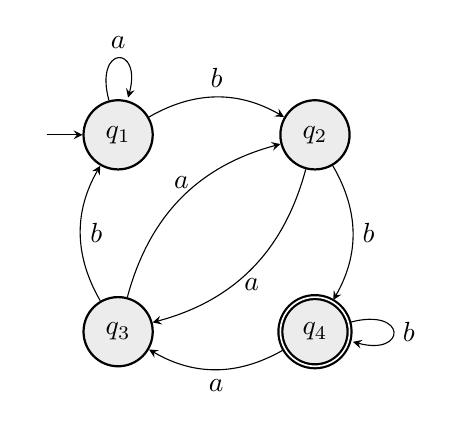
\begin{tikzpicture}
                  \node[state, initial] (q1) {$q_1$};
                  \node[state, right of=q1] (q2) {$q_2$};
                  \node[state, below of=q1] (q3) {$q_3$};
                  \node[state, accepting, below of=q2] (q4) {$q_4$};
                  \draw (q1) edge[loop above] node{$a$} (q1)
                  (q1) edge[bend left, above] node{$b$} (q2)
                  (q2) edge[bend left, below] node{$a$} (q3)
                  (q2) edge[bend left, right] node{$b$} (q4)
                  (q3) edge[bend left, above] node{$a$} (q2)
                  (q3) edge[bend left, right] node{$b$} (q1)
                  (q4) edge[bend left, below] node{$a$} (q3)
                  (q4) edge[loop right] node{$b$} (q4);
              \end{tikzpicture}
              \caption{$M_1$ and $M_2$}
          \end{figure}

          \begin{enumerate}
              \item What is the start state?

                    $M_1: q_1$

                    $M_2: q_1$

              \item What is the set of accept states?

                    $M_1: \{q_2\}$

                    $M_2: \{q_4\}$
              \item What sequence of states does the machine go through on input $aabb$?

                    $M_1: q_1 \rightarrow q_2 \rightarrow q_3 \rightarrow q_1 \rightarrow q_1$

                    $M_2: q_1 \rightarrow q_2 \rightarrow q_4 \rightarrow q_4 \rightarrow q_4$
              \item Does the machine accept the string $aabb$?

                    $M_1:$ No

                    $M_2:$ Yes
              \item Does the machine accept the string $\epsilon$?

                    $M_1:$ No

                    $M_2:$ No
          \end{enumerate}

    \item[1.2]

          Give the formal description of the machines $M_1$ and $M_2$ pictured in Exercise 1.1.

          $M_1 = (Q, \Sigma_1, \delta_1, q_1, \{q_2\})$

          $Q = \{q_1, q_2, q_3\}$

          $\Sigma_1 = \{a, b\}$

          $\delta_1 = \{((q_1, a), q_2), ((q_1, b), q_1), ((q_2, a), q_3), ((q_2, b), q_3), ((q_3, a), q_2), ((q_3, b), q_1)\}$\\

          $M_2 = (Q, \Sigma_2, \delta_2, q_1, \{q_4\})$

          $Q = \{q_1, q_2, q_3, q_4\}$

          $\Sigma_2 = \{a, b\}$

          $\delta_2 = \{((q_1, a), q_1), ((q_1, b), q_2), ((q_2, a), q_3), ((q_2, b), q_4),$\\
          .\,\,\,\qquad$((q_3, a), q_2), ((q_3, b), q_1), ((q_4, a), q_3), ((q_4, b), q_4)\}$

    \item[1.3]

          The formal description of a DFA $M$ is $\{q_1,q_2,q_3,q_4,q_5\},\{u,d\},\sigma,q_3,\{q_3\}$, where $\sigma$ is given by the following table. Give the state diagram of this machine.

          \begin{center}


              \begin{tabular}{ c | c c }
                        & $u$   & $d$   \\
                  \hline
                  $q_1$ & $q_1$ & $q_2$ \\
                  $q_2$ & $q_1$ & $q_3$ \\
                  $q_3$ & $q_2$ & $q_4$ \\
                  $q_4$ & $q_3$ & $q_5$ \\
                  $q_5$ & $q_4$ & $q_5$ \\
              \end{tabular}
          \end{center}

          \begin{figure}[H]
              \centering
              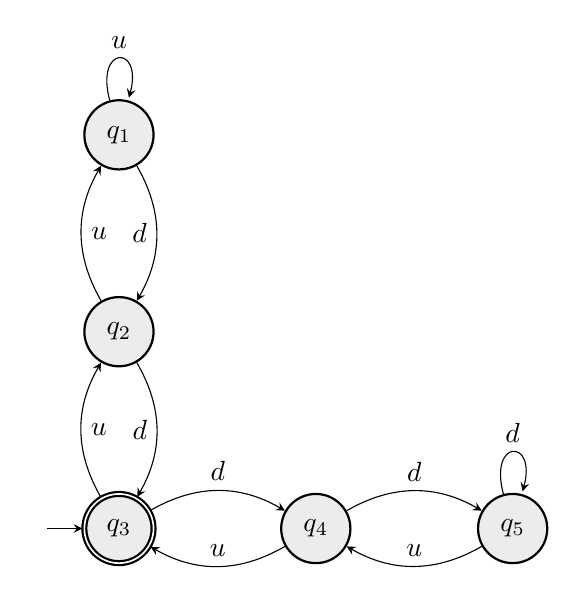
\begin{tikzpicture}
                  \node[state] (q1) {$q_1$};
                  \node[state, below of=q1] (q2) {$q_2$};
                  \node[state, accepting, initial, below of=q2] (q3) {$q_3$};
                  \node[state, right of=q3] (q4) {$q_4$};
                  \node[state, right of=q4] (q5) {$q_5$};
                  \draw (q1) edge[loop above] node{$u$} (q1)
                  (q1) edge[bend left, left] node{$d$} (q2)
                  (q2) edge[bend left, right] node{$u$} (q1)
                  (q2) edge[bend left, left] node{$d$} (q3)
                  (q3) edge[bend left, right] node{$u$} (q2)
                  (q3) edge[bend left, above] node{$d$} (q4)
                  (q4) edge[bend left, above] node{$u$} (q3)
                  (q4) edge[bend left, above] node{$d$} (q5)
                  (q5) edge[loop above] node{$d$} (q5)
                  (q5) edge[bend left, above] node{$u$} (q4);
              \end{tikzpicture}
          \end{figure}

    \item[1.4]
          Each of the following languages is the intersection of two simpler languages. In each part, construct DFAs for the simpler languages,then combine them using the construction discussed in footnote 3 (page 46) to give the state diagram of a DFA for the language given. In all parts, $\Sigma=\{a,b\}$.
          \begin{enumerate}
              \item $\{w|w~\text{has at least three }a\text{’s and at least two }b\text{’s}\}$

                    $DFA_1$ for at least three $a$'s:

                    \begin{figure}[H]
                        \centering
                        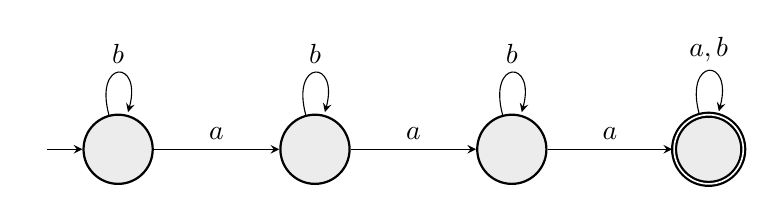
\begin{tikzpicture}
                            \node[state, initial] (q1) {};
                            \node[state, right of=q1] (q2) {};
                            \node[state, right of=q2] (q3) {};
                            \node[state, right of=q3, accepting] (q4) {};
                            \draw (q1) edge[loop above] node{$b$} (q1)
                            (q2) edge[loop above] node{$b$} (q2)
                            (q3) edge[loop above] node{$b$} (q3)
                            (q4) edge[loop above] node{$a,b$} (q4)
                            (q1) edge[left, above] node{$a$} (q2)
                            (q2) edge[left, above] node{$a$} (q3)
                            (q3) edge[left, above] node{$a$} (q4);
                        \end{tikzpicture}
                    \end{figure}

                    $DFA_2$ for at least two $b$'s:

                    \begin{figure}[H]
                        \centering
                        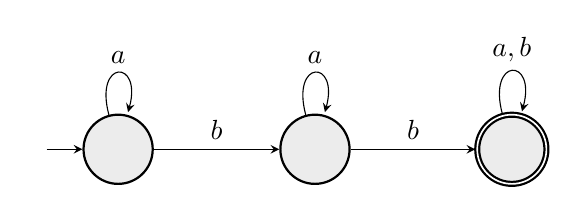
\begin{tikzpicture}
                            \node[state, initial] (q1) {};
                            \node[state, right of=q1] (q2) {};
                            \node[state, right of=q2, accepting] (q3) {};
                            \draw (q1) edge[loop above] node{$a$} (q1)
                            (q2) edge[loop above] node{$a$} (q2)
                            (q3) edge[loop above] node{$a,b$} (q3)
                            (q1) edge[left, above] node{$b$} (q2)
                            (q2) edge[left, above] node{$b$} (q3);
                        \end{tikzpicture}
                    \end{figure}

                    $DFA$ for at least three $a$'s and at least two $b$'s:

                    \begin{figure}[H]
                        \centering
                        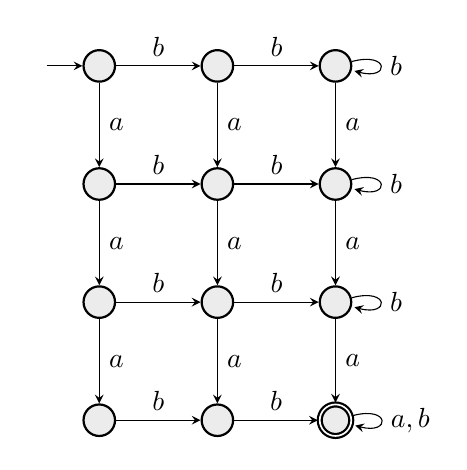
\begin{tikzpicture}[
                                styleSmall/.style={minimum size=4mm},
                                node distance=1.5cm,
                            ]
                            \node[state, initial, styleSmall] (q11) {};
                            \node[state, right of=q11, styleSmall] (q12) {};
                            \node[state, right of=q12, styleSmall] (q13) {};
                            \node[state, below of=q11, styleSmall] (q21) {};
                            \node[state, below of=q12, styleSmall] (q22) {};
                            \node[state, below of=q13, styleSmall] (q23) {};
                            \node[state, below of=q21, styleSmall] (q31) {};
                            \node[state, below of=q22, styleSmall] (q32) {};
                            \node[state, below of=q23, styleSmall] (q33) {};
                            \node[state, below of=q31, styleSmall] (q41) {};
                            \node[state, below of=q32, styleSmall] (q42) {};
                            \node[state, below of=q33, styleSmall, accepting] (q43) {};
                            \draw
                            (q13) edge[loop right] node{$b$} (q13)

                            (q11) edge[left, above] node{$b$} (q12)
                            (q12) edge[left, above] node{$b$} (q13)
                            (q23) edge[loop right] node{$b$} (q23)
                            (q21) edge[left, above] node{$b$} (q22)
                            (q22) edge[left, above] node{$b$} (q23)
                            (q33) edge[loop right] node{$b$} (q33)
                            (q31) edge[left, above] node{$b$} (q32)
                            (q32) edge[left, above] node{$b$} (q33)
                            (q43) edge[loop right] node{$a,b$} (q43)
                            (q41) edge[left, above] node{$b$} (q42)
                            (q42) edge[left, above] node{$b$} (q43)

                            (q11) edge[left, right] node{$a$} (q21)
                            (q12) edge[left, right] node{$a$} (q22)
                            (q13) edge[left, right] node{$a$} (q23)
                            (q21) edge[left, right] node{$a$} (q31)
                            (q22) edge[left, right] node{$a$} (q32)
                            (q23) edge[left, right] node{$a$} (q33)
                            (q31) edge[left, right] node{$a$} (q41)
                            (q32) edge[left, right] node{$a$} (q42)
                            (q33) edge[left, right] node{$a$} (q43);
                        \end{tikzpicture}
                    \end{figure}

              \item $\{w|w~\text{has exactly two }a\text{’s and at least two }b\text{’s}\}$

                    $DFA_1$ for exactly two $a$'s:

                    \begin{figure}[H]
                        \centering
                        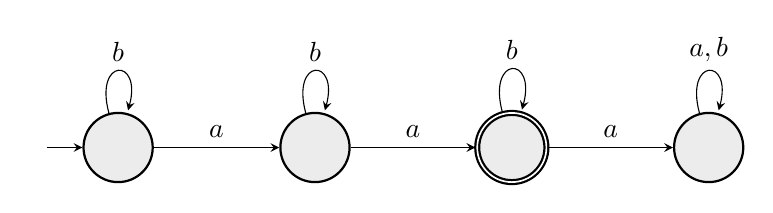
\begin{tikzpicture}
                            \node[state, initial] (q1) {};
                            \node[state, right of=q1] (q2) {};
                            \node[state, right of=q2, accepting] (q3) {};
                            \node[state, right of=q3] (q4) {};
                            \draw (q1) edge[loop above] node{$b$} (q1)
                            (q2) edge[loop above] node{$b$} (q2)
                            (q3) edge[loop above] node{$b$} (q3)
                            (q4) edge[loop above] node{$a,b$} (q4)
                            (q1) edge[left, above] node{$a$} (q2)
                            (q2) edge[left, above] node{$a$} (q3)
                            (q3) edge[left, above] node{$a$} (q4);
                        \end{tikzpicture}
                    \end{figure}

                    $DFA_2$ for at least two $b$'s:

                    \begin{figure}[H]
                        \centering
                        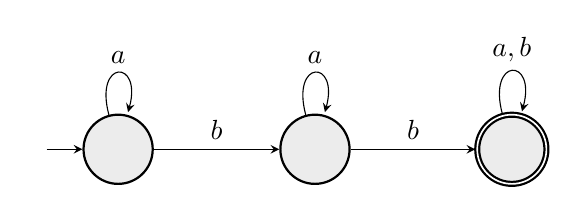
\begin{tikzpicture}
                            \node[state, initial] (q1) {};
                            \node[state, right of=q1] (q2) {};
                            \node[state, right of=q2, accepting] (q3) {};
                            \draw (q1) edge[loop above] node{$a$} (q1)
                            (q2) edge[loop above] node{$a$} (q2)
                            (q3) edge[loop above] node{$a,b$} (q3)
                            (q1) edge[left, above] node{$b$} (q2)
                            (q2) edge[left, above] node{$b$} (q3);
                        \end{tikzpicture}
                    \end{figure}

                    $DFA$ for exactly two $a$'s and at least two $b$'s:

                    \begin{figure}[H]
                        \centering
                        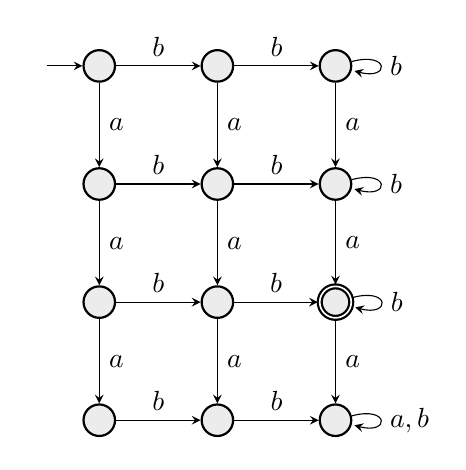
\begin{tikzpicture}[
                                styleSmall/.style={minimum size=4mm},
                                node distance=1.5cm,
                            ]
                            \node[state, initial, styleSmall] (q11) {};
                            \node[state, right of=q11, styleSmall] (q12) {};
                            \node[state, right of=q12, styleSmall] (q13) {};
                            \node[state, below of=q11, styleSmall] (q21) {};
                            \node[state, below of=q12, styleSmall] (q22) {};
                            \node[state, below of=q13, styleSmall] (q23) {};
                            \node[state, below of=q21, styleSmall] (q31) {};
                            \node[state, below of=q22, styleSmall] (q32) {};
                            \node[state, below of=q23, styleSmall, accepting] (q33) {};
                            \node[state, below of=q31, styleSmall] (q41) {};
                            \node[state, below of=q32, styleSmall] (q42) {};
                            \node[state, below of=q33, styleSmall] (q43) {};
                            \draw
                            (q13) edge[loop right] node{$b$} (q13)
                            (q11) edge[left, above] node{$b$} (q12)
                            (q12) edge[left, above] node{$b$} (q13)
                            (q23) edge[loop right] node{$b$} (q23)
                            (q21) edge[left, above] node{$b$} (q22)
                            (q22) edge[left, above] node{$b$} (q23)
                            (q33) edge[loop right] node{$b$} (q33)
                            (q31) edge[left, above] node{$b$} (q32)
                            (q32) edge[left, above] node{$b$} (q33)
                            (q43) edge[loop right] node{$a,b$} (q43)
                            (q41) edge[left, above] node{$b$} (q42)
                            (q42) edge[left, above] node{$b$} (q43)

                            (q11) edge[left, right] node{$a$} (q21)
                            (q12) edge[left, right] node{$a$} (q22)
                            (q13) edge[left, right] node{$a$} (q23)
                            (q21) edge[left, right] node{$a$} (q31)
                            (q22) edge[left, right] node{$a$} (q32)
                            (q23) edge[left, right] node{$a$} (q33)
                            (q31) edge[left, right] node{$a$} (q41)
                            (q32) edge[left, right] node{$a$} (q42)
                            (q33) edge[left, right] node{$a$} (q43);
                        \end{tikzpicture}
                    \end{figure}

              \item $\{w|w~\text{has an even number of }a\text{’s and one or two }b\text{’s}\}$

                    $DFA_1$ for an even number of $a$'s:

                    \begin{figure}[H]
                        \centering
                        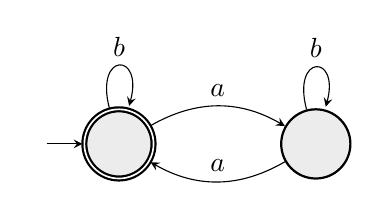
\begin{tikzpicture}
                            \node[state, initial, accepting] (q1) {};
                            \node[state, right of=q1] (q2) {};
                            \draw (q1) edge[loop above] node{$b$} (q1)
                            (q2) edge[loop above] node{$b$} (q2)
                            (q1) edge[bend left, above] node{$a$} (q2)
                            (q2) edge[bend left, above] node{$a$} (q1);
                        \end{tikzpicture}
                    \end{figure}

                    $DFA_2$ for one or two $b$'s:

                    \begin{figure}[H]
                        \centering
                        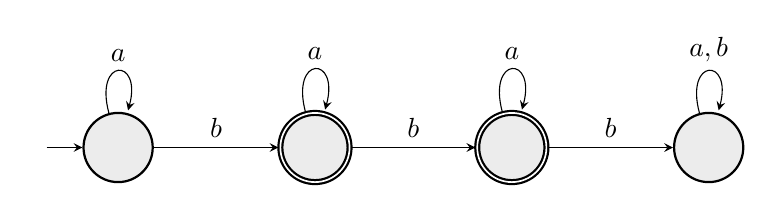
\begin{tikzpicture}
                            \node[state, initial] (q1) {};
                            \node[state, right of=q1, accepting] (q2) {};
                            \node[state, right of=q2, accepting] (q3) {};
                            \node[state, right of=q3] (q4) {};
                            \draw (q1) edge[loop above] node{$a$} (q1)
                            (q2) edge[loop above] node{$a$} (q2)
                            (q3) edge[loop above] node{$a$} (q3)
                            (q4) edge[loop above] node{$a,b$} (q4)
                            (q1) edge[left, above] node{$b$} (q2)
                            (q2) edge[left, above] node{$b$} (q3)
                            (q3) edge[left, above] node{$b$} (q4);
                        \end{tikzpicture}
                    \end{figure}

                    $DFA$ for an even number of $a$'s and one or two $b$'s:

                    \begin{figure}[H]
                        \centering
                        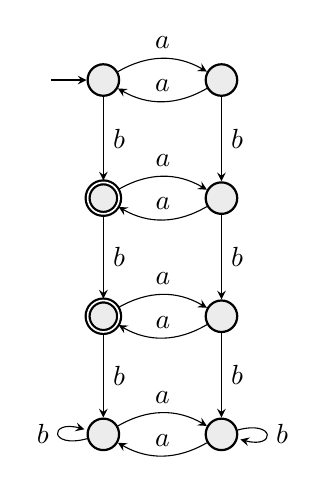
\begin{tikzpicture}[
                                styleSmall/.style={minimum size=4mm},
                                node distance=1.5cm,
                            ]
                            \node[state, initial, styleSmall] (q11) {};
                            \node[state, right of=q11, styleSmall] (q12) {};
                            \node[state, below of=q11, styleSmall, accepting] (q21) {};
                            \node[state, below of=q12, styleSmall] (q22) {};
                            \node[state, below of=q21, styleSmall, accepting] (q31) {};
                            \node[state, below of=q22, styleSmall] (q32) {};
                            \node[state, below of=q31, styleSmall] (q41) {};
                            \node[state, below of=q32, styleSmall] (q42) {};
                            \draw
                            (q11) edge[bend left, above] node{$a$} (q12)
                            (q12) edge[bend left, above] node{$a$} (q11)
                            (q21) edge[bend left, above] node{$a$} (q22)
                            (q22) edge[bend left, above] node{$a$} (q21)
                            (q31) edge[bend left, above] node{$a$} (q32)
                            (q32) edge[bend left, above] node{$a$} (q31)
                            (q41) edge[bend left, above] node{$a$} (q42)
                            (q42) edge[bend left, above] node{$a$} (q41)

                            (q41) edge[loop left] node{$b$} (q41)
                            (q42) edge[loop right] node{$b$} (q42)

                            (q11) edge[left, right] node{$b$} (q21)
                            (q12) edge[left, right] node{$b$} (q22)
                            (q21) edge[left, right] node{$b$} (q31)
                            (q22) edge[left, right] node{$b$} (q32)
                            (q31) edge[left, right] node{$b$} (q41)
                            (q32) edge[left, right] node{$b$} (q42);
                        \end{tikzpicture}
                    \end{figure}


              \item $\{w|w~\text{has an even number of }a\text{’s and each }a\text{ is followed by at least one }b\}$

                    $DFA_1$ for an even number of $a$'s:

                    \begin{figure}[H]
                        \centering
                        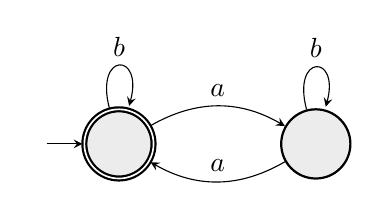
\begin{tikzpicture}
                            \node[state, initial, accepting] (q1) {};
                            \node[state, right of=q1] (q2) {};
                            \draw (q1) edge[loop above] node{$b$} (q1)
                            (q2) edge[loop above] node{$b$} (q2)
                            (q1) edge[bend left, above] node{$a$} (q2)
                            (q2) edge[bend left, above] node{$a$} (q1);
                        \end{tikzpicture}
                    \end{figure}

                    $DFA_2$ for each $a$ is followed by at least one $b$:

                    \begin{figure}[H]
                        \centering
                        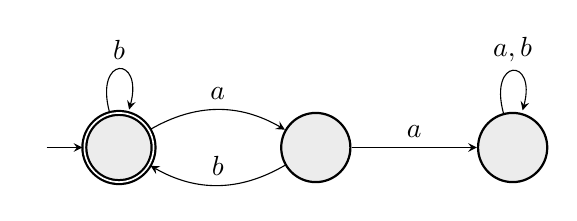
\begin{tikzpicture}
                            \node[state, initial, accepting] (q1) {};
                            \node[state, right of=q1] (q2) {};
                            \node[state, right of=q2] (q3) {};
                            \draw (q1) edge[loop above] node{$b$} (q1)
                            (q3) edge[loop above] node{$a,b$} (q3)
                            (q1) edge[bend left, above] node{$a$} (q2)
                            (q2) edge[bend left, above] node{$b$} (q1)
                            (q2) edge[left, above] node{$a$} (q3);
                        \end{tikzpicture}
                    \end{figure}

                    $DFA$ for an even number of $a$'s and each $a$ is followed by at least one $b$:

                    \begin{figure}[H]
                        \centering
                        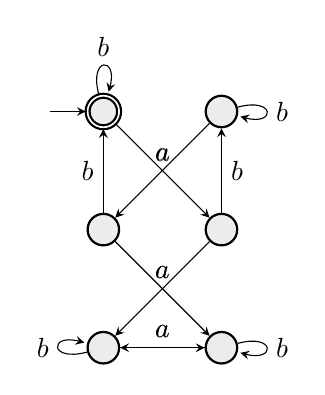
\begin{tikzpicture}[
                                styleSmall/.style={minimum size=4mm},
                                node distance=1.5cm,
                            ]
                            \node[state, initial, styleSmall, accepting] (q11) {};
                            \node[state, below of=q11, styleSmall] (q12) {};
                            \node[state, below of=q12, styleSmall] (q13) {};
                            \node[state, right of=q11, styleSmall] (q21) {};
                            \node[state, below of=q21, styleSmall] (q22) {};
                            \node[state, below of=q22, styleSmall] (q23) {};
                            \draw
                            (q11) edge[left, above] node{$a$} (q22)
                            (q11) edge[loop above] node{$b$} (q11)
                            (q12) edge[left, above] node{$a$} (q23)
                            (q12) edge[left, left] node{$b$} (q11)
                            (q13) edge[left, above] node{$a$} (q23)
                            (q13) edge[loop left] node{$b$} (q13)

                            (q21) edge[left, above] node{$a$} (q12)
                            (q21) edge[loop right] node{$b$} (q21)
                            (q22) edge[left, above] node{$a$} (q13)
                            (q22) edge[left, right] node{$b$} (q21)
                            (q23) edge[left, above] node{$a$} (q13)
                            (q23) edge[loop right] node{$b$} (q23);
                        \end{tikzpicture}
                    \end{figure}

              \item $\{w|w~\text{starts with an }a\text{ and has at most one }b\}$

                    $DFA_1$ for starts with an $a$:

                    \begin{figure}[H]
                        \centering
                        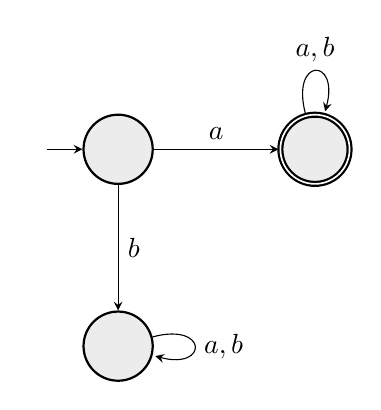
\begin{tikzpicture}
                            \node[state, initial] (q1) {};
                            \node[state, right of=q1, accepting] (q2) {};
                            \node[state, below of=q1 ] (q3) {};
                            \draw
                            (q3) edge[loop right] node{$a,b$} (q3)
                            (q2) edge[loop above] node{$a,b$} (q2)
                            (q1) edge[above] node{$a$} (q2)
                            (q1) edge[right] node{$b$} (q3);
                        \end{tikzpicture}
                    \end{figure}

                    $DFA_2$ for has at most one $b$:

                    \begin{figure}[H]
                        \centering
                        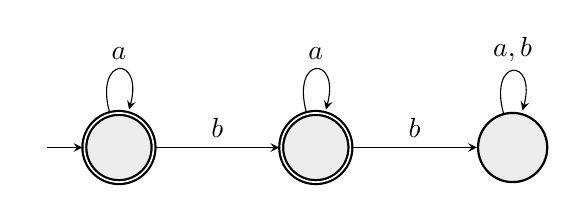
\begin{tikzpicture}
                            \node[state, initial, accepting] (q1) {};
                            \node[state, right of=q1, accepting] (q2) {};
                            \node[state, right of=q2] (q3) {};
                            \draw (q1) edge[loop above] node{$a$} (q1)
                            (q2) edge[loop above] node{$a$} (q2)
                            (q3) edge[loop above] node{$a,b$} (q3)
                            (q1) edge[left, above] node{$b$} (q2)
                            (q2) edge[left, above] node{$b$} (q3);
                        \end{tikzpicture}
                    \end{figure}

              \item $\{w|w~\text{has an odd number of }a\text{’s and ends with a }b\}$

                    $DFA_1$ for an odd number of $a$'s:

                    \begin{figure}[H]
                        \centering
                        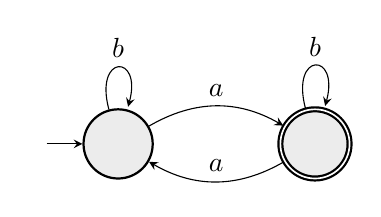
\begin{tikzpicture}
                            \node[state, initial] (q1) {};
                            \node[state, right of=q1, accepting] (q2) {};
                            \draw (q1) edge[loop above] node{$b$} (q1)
                            (q2) edge[loop above] node{$b$} (q2)
                            (q1) edge[bend left, above] node{$a$} (q2)
                            (q2) edge[bend left, above] node{$a$} (q1);
                        \end{tikzpicture}
                    \end{figure}

                    $DFA_2$ for ends with a $b$:

                    \begin{figure}[H]
                        \centering
                        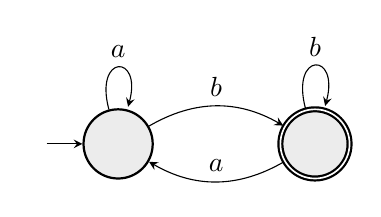
\begin{tikzpicture}
                            \node[state, initial] (q1) {};
                            \node[state, right of=q1, accepting] (q2) {};
                            \draw (q1) edge[loop above] node{$a$} (q1)
                            (q2) edge[loop above] node{$b$} (q2)
                            (q1) edge[bend left, above] node{$b$} (q2)
                            (q2) edge[bend left, above] node{$a$} (q1);
                        \end{tikzpicture}
                    \end{figure}

                    $DFA$ for an odd number of $a$'s and ends with a $b$:

                    \begin{figure}[H]
                        \centering
                        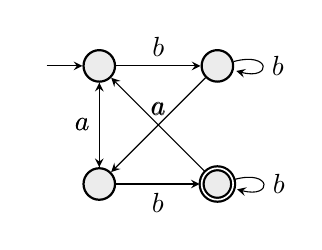
\begin{tikzpicture}[
                                styleSmall/.style={minimum size=4mm},
                                node distance=1.5cm,
                            ]
                            \node[state, initial, styleSmall] (q11) {};
                            \node[state, right of=q11, styleSmall] (q12) {};
                            \node[state, below of=q11, styleSmall] (q21) {};
                            \node[state, below of=q12, styleSmall, accepting] (q22) {};
                            \draw
                            (q11) edge[left, above] node{$b$} (q12)
                            (q21) edge[left, below] node{$b$} (q22)
                            (q12) edge[loop right] node{$b$} (q12)
                            (q22) edge[loop right] node{$b$} (q22)
                            (q11) edge[left, left] node{$a$} (q21)
                            (q22) edge[left, above] node{$a$} (q11)
                            (q21) edge[left, left] node{$a$} (q11)
                            (q12) edge[left, above] node{$a$} (q21);
                        \end{tikzpicture}
                    \end{figure}

              \item $\{w|w~\text{has even length and an odd number of }a\text{’s}\}$

                    $DFA_1$ for even length:

                    \begin{figure}[H]
                        \centering
                        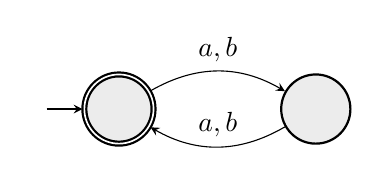
\begin{tikzpicture}
                            \node[state, initial, accepting] (q1) {};
                            \node[state, right of=q1] (q2) {};
                            \draw
                            (q1) edge[bend left, above] node{$a,b$} (q2)
                            (q2) edge[bend left, above] node{$a,b$} (q1);
                        \end{tikzpicture}
                    \end{figure}

                    $DFA_2$ for an odd number of $a$'s:

                    \begin{figure}[H]
                        \centering
                        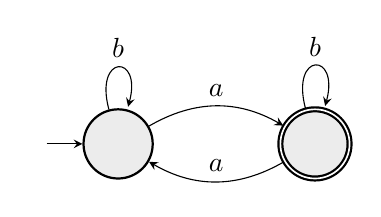
\begin{tikzpicture}
                            \node[state, initial] (q1) {};
                            \node[state, right of=q1, accepting] (q2) {};
                            \draw (q1) edge[loop above] node{$b$} (q1)
                            (q2) edge[loop above] node{$b$} (q2)
                            (q1) edge[bend left, above] node{$a$} (q2)
                            (q2) edge[bend left, above] node{$a$} (q1);
                        \end{tikzpicture}
                    \end{figure}

                    $DFA$ for even length and an odd number of $a$'s:

                    \begin{figure}[H]
                        \centering
                        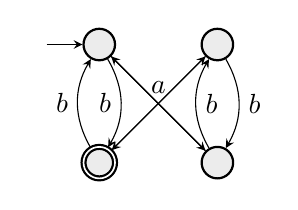
\begin{tikzpicture}[
                                styleSmall/.style={minimum size=4mm},
                                node distance=1.5cm,
                            ]
                            \node[state, initial, styleSmall] (q11) {};
                            \node[state, right of=q11, styleSmall] (q12) {};
                            \node[state, below of=q11, styleSmall, accepting] (q21) {};
                            \node[state, below of=q12, styleSmall] (q22) {};
                            \draw
                            (q11) edge[bend left, left] node{$b$} (q21)
                            (q21) edge[bend left, left] node{$b$} (q11)
                            (q12) edge[bend left, right] node{$b$} (q22)
                            (q22) edge[bend left, right] node{$b$} (q12)
                            (q11) edge[left, above] node{$a$} (q22)
                            (q22) edge[left, above] node{} (q11)
                            (q21) edge[left, above] node{} (q12)
                            (q12) edge[left, above] node{} (q21);
                        \end{tikzpicture}
                    \end{figure}

          \end{enumerate}

    \item[1.5]
          Each of the following languages is the complement of a simpler language. In each part, construct a DFA for the simpler language, then use it to give the state diagram of a DFA for the language given. In all parts, $\Sigma=\{a,b\}$.
          \begin{enumerate}
              \item $A = \{w|w~\text{does not contain the substring }ab\}$

                    $\overline{A} = \{w|w~\text{contains the substring }ab\}$
                    \begin{figure}[H]
                        \centering
                        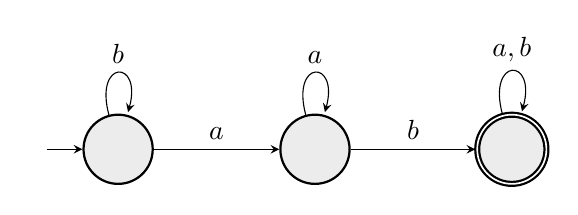
\begin{tikzpicture}
                            \node[state, initial] (q1) {};
                            \node[state, right of=q1] (q2) {};
                            \node[state, accepting, right of=q2] (q3) {};
                            \draw (q1) edge[left, above] node{$a$} (q2)
                            (q1) edge[loop above] node{$b$} (q1)
                            (q2) edge[left, above] node{$b$} (q3)
                            (q2) edge[loop above] node{$a$} (q2)
                            (q3) edge[loop above] node{$a,b$} (q3);
                        \end{tikzpicture}
                        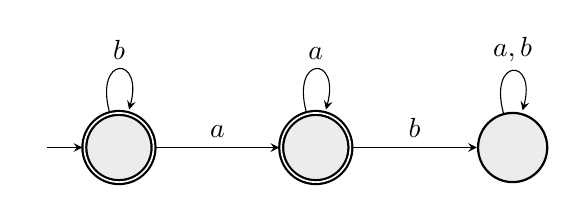
\begin{tikzpicture}
                            \node[state, accepting, initial] (q1) {};
                            \node[state, accepting, right of=q1] (q2) {};
                            \node[state, right of=q2] (q3) {};
                            \draw (q1) edge[left, above] node{$a$} (q2)
                            (q1) edge[loop above] node{$b$} (q1)
                            (q2) edge[left, above] node{$b$} (q3)
                            (q2) edge[loop above] node{$a$} (q2)
                            (q3) edge[loop above] node{$a,b$} (q3);
                        \end{tikzpicture}
                        \caption{$\overline{A}$ and $A$}
                    \end{figure}
              \item $B = \{w|w~\text{does notcontain the substring }baba\}$

                    $\overline{B} = \{w|w~\text{contains the substring }baba\}$
                    \begin{figure}[H]
                        \centering
                        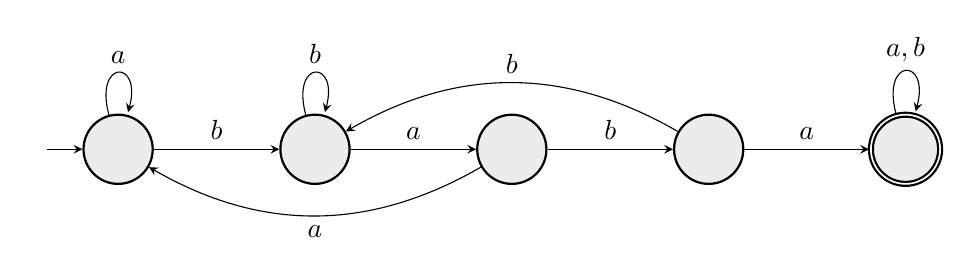
\begin{tikzpicture}
                            \node[state, initial] (q1) {};
                            \node[state, right of=q1] (q2) {};
                            \node[state, right of=q2] (q3) {};
                            \node[state, right of=q3] (q4) {};
                            \node[state, accepting, right of=q4] (q5) {};
                            \draw (q1) edge[left, above] node{$b$} (q2)
                            (q1) edge[loop above] node{$a$} (q1)
                            (q2) edge[left, above] node{$a$} (q3)
                            (q2) edge[loop above] node{$b$} (q2)
                            (q3) edge[left, above] node{$b$} (q4)
                            (q3) edge[bend left, below] node{$a$} (q1)
                            (q4) edge[bend right, above] node{$b$} (q2)
                            (q4) edge[left, above] node{$a$} (q5)
                            (q5) edge[loop above] node{$a,b$} (q5);
                        \end{tikzpicture}
                        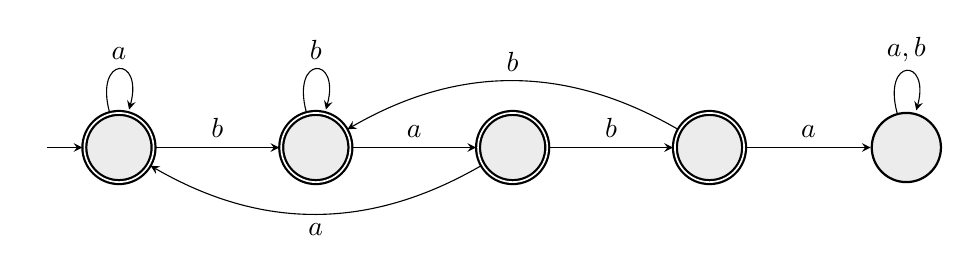
\begin{tikzpicture}
                            \node[state, accepting, initial] (q1) {};
                            \node[state, accepting, right of=q1] (q2) {};
                            \node[state, accepting, right of=q2] (q3) {};
                            \node[state, accepting, right of=q3] (q4) {};
                            \node[state, right of=q4] (q5) {};
                            \draw (q1) edge[left, above] node{$b$} (q2)
                            (q1) edge[loop above] node{$a$} (q1)
                            (q2) edge[left, above] node{$a$} (q3)
                            (q2) edge[loop above] node{$b$} (q2)
                            (q3) edge[left, above] node{$b$} (q4)
                            (q3) edge[bend left, below] node{$a$} (q1)
                            (q4) edge[bend right, above] node{$b$} (q2)
                            (q4) edge[left, above] node{$a$} (q5)
                            (q5) edge[loop above] node{$a,b$} (q5);
                        \end{tikzpicture}
                        \caption{$\overline{B}$ and $B$}
                    \end{figure}

              \item $C =\{w|w~\text{contains neither the substrings }ab\text{ nor }ba\}$

                    $\overline{C} = \{w|w~\text{contains the substring }ab\text{ or }ba\}$
                    \begin{figure}[H]
                        \centering
                        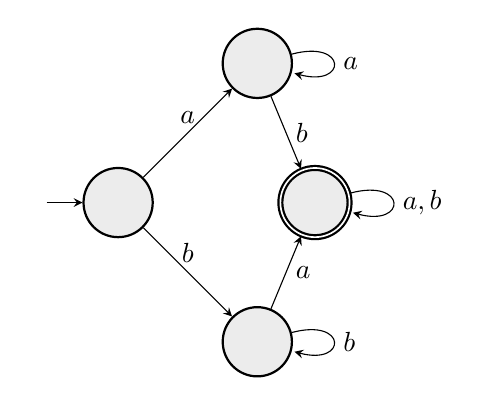
\begin{tikzpicture}
                            \node[state, initial] (q1) {};
                            \node[state, above right of=q1] (q2) {};
                            \node[state, below right of=q1] (q3) {};
                            \node[state, accepting, right of=q1] (q4) {};
                            \draw (q1) edge[left, above] node{$a$} (q2)
                            (q1) edge[left, above] node{$b$} (q3)
                            (q2) edge[right] node{$b$} (q4)
                            (q2) edge[loop right] node{$a$} (q2)
                            (q3) edge[right] node{$a$} (q4)
                            (q3) edge[loop right] node{$b$} (q3)
                            (q4) edge[loop right] node{$a,b$} (q4);
                        \end{tikzpicture}
                        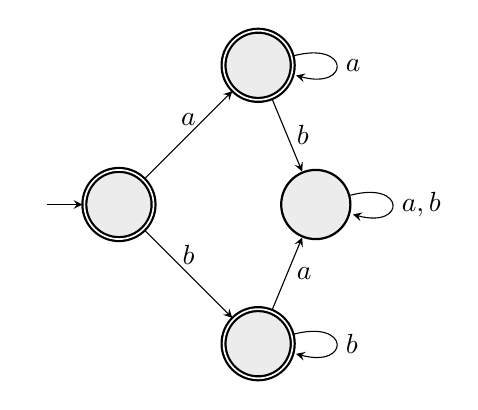
\begin{tikzpicture}
                            \node[state, accepting, initial] (q1) {};
                            \node[state, accepting, above right of=q1] (q2) {};
                            \node[state, accepting, below right of=q1] (q3) {};
                            \node[state, right of=q1] (q4) {};
                            \draw (q1) edge[left, above] node{$a$} (q2)
                            (q1) edge[left, above] node{$b$} (q3)
                            (q2) edge[right] node{$b$} (q4)
                            (q2) edge[loop right] node{$a$} (q2)
                            (q3) edge[right] node{$a$} (q4)
                            (q3) edge[loop right] node{$b$} (q3)
                            (q4) edge[loop right] node{$a,b$} (q4);
                        \end{tikzpicture}
                        \caption{$\overline{C}$ and $C$}
                    \end{figure}
              \item $D = \{w|w~\text{is any string not in }a^{\ast}b^{\ast}\}$

                    $\overline{D} = \{w|w~\text{is any string in }a^{\ast}b^{\ast}\}$
                    \begin{figure}[H]
                        \centering
                        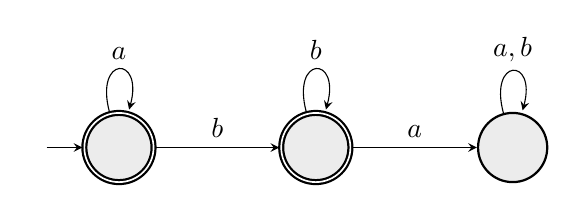
\begin{tikzpicture}
                            \node[state, accepting, initial] (q1) {};
                            \node[state, accepting, right of=q1] (q2) {};
                            \node[state, right of=q2] (q3) {};
                            \draw (q1) edge[loop above] node{$a$} (q1)
                            (q1) edge[above] node{$b$} (q2)
                            (q2) edge[loop above] node{$b$} (q2)
                            (q2) edge[above] node{$a$} (q3)
                            (q3) edge[loop above] node{$a,b$} (q3);
                        \end{tikzpicture}
                        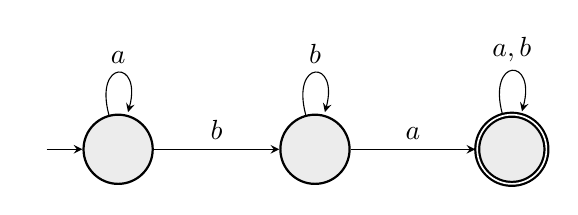
\begin{tikzpicture}
                            \node[state, initial] (q1) {};
                            \node[state, right of=q1] (q2) {};
                            \node[state, accepting, right of=q2] (q3) {};
                            \draw (q1) edge[loop above] node{$a$} (q1)
                            (q1) edge[above] node{$b$} (q2)
                            (q2) edge[loop above] node{$b$} (q2)
                            (q2) edge[above] node{$a$} (q3)
                            (q3) edge[loop above] node{$a,b$} (q3);
                        \end{tikzpicture}
                        \caption{$\overline{D}$ and $D$}
                    \end{figure}
              \item $E = \{w|w~\text{is any string not in }(ab^+)^{\ast}\}$

                    $\overline{E} = \{w|w~\text{is any string in }(ab^+)^{\ast}\}$

                    \begin{itemize}
                        \item assuming $ab^+$ means $a$ followed by one or more $b$.
                              \begin{figure}[H]
                                  \centering
                                  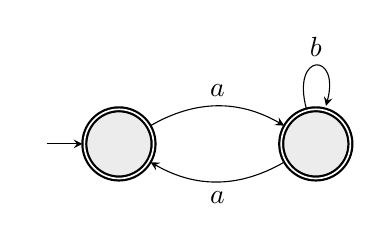
\begin{tikzpicture}
                                      \node[state, accepting, initial] (q1) {};
                                      \node[state, accepting, right of=q1] (q2) {};
                                      \draw (q1) edge[bend left, above] node{$a$} (q2)
                                      (q2) edge[bend left, below] node{$a$} (q1)
                                      (q2) edge[loop above] node{$b$} (q2);
                                  \end{tikzpicture}
                                  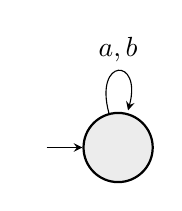
\begin{tikzpicture}
                                      \node[state, initial] (q1) {};
                                      \draw (q1) edge[loop above] node{$a,b$} (q1);
                                  \end{tikzpicture}
                                  \caption{$\overline{E}$ and $E$}
                              \end{figure}
                        \item assuming $ab^+$ means $ab$ one or more times.
                              \begin{figure}[H]
                                  \centering
                                  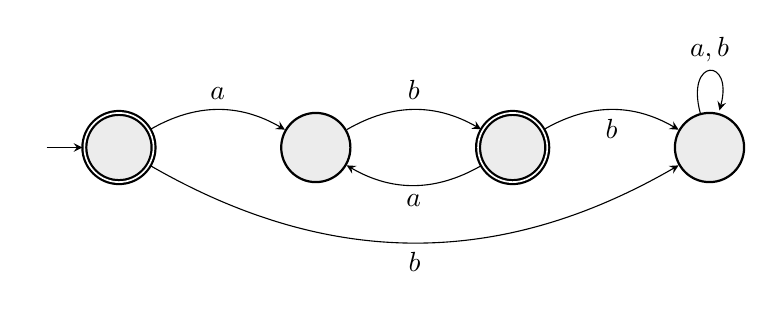
\begin{tikzpicture}
                                      \node[state, accepting, initial] (q1) {};
                                      \node[state, right of=q1] (q2) {};
                                      \node[state, accepting, right of=q2] (q3) {};
                                      \node[state, right of=q3] (q4) {};
                                      \draw (q1) edge[bend left, above] node{$a$} (q2)
                                      (q2) edge[bend left, above] node{$b$} (q3)
                                      (q3) edge[bend left, below] node{$a$} (q2)
                                      (q3) edge[bend left, below] node{$b$} (q4)
                                      (q1) edge[bend right, below] node{$b$} (q4)
                                      (q4) edge[loop above] node{$a,b$} (q4);
                                  \end{tikzpicture}
                                  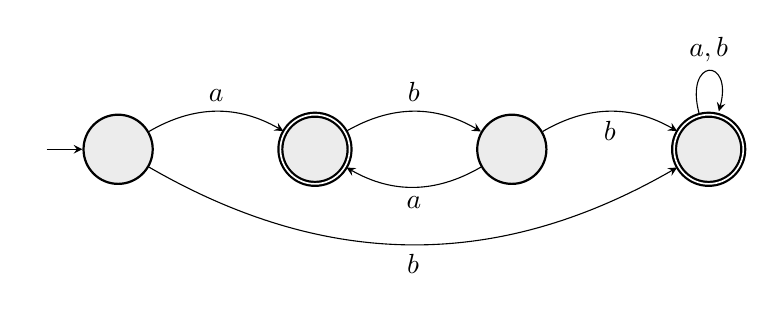
\begin{tikzpicture}
                                      \node[state, initial] (q1) {};
                                      \node[state, accepting, right of=q1] (q2) {};
                                      \node[state, right of=q2] (q3) {};
                                      \node[state, accepting, right of=q3] (q4) {};
                                      \draw (q1) edge[bend left, above] node{$a$} (q2)
                                      (q2) edge[bend left, above] node{$b$} (q3)
                                      (q3) edge[bend left, below] node{$a$} (q2)
                                      (q3) edge[bend left, below] node{$b$} (q4)
                                      (q1) edge[bend right, below] node{$b$} (q4)
                                      (q4) edge[loop above] node{$a,b$} (q4);
                                  \end{tikzpicture}
                                  \caption{$\overline{E}$ and $E$}
                              \end{figure}
                    \end{itemize}
              \item $F = \{w|w~\text{is any string not in }a^{\ast} \cup b^{\ast}\}$

                    $\overline{F} = \{w|w~\text{is any string in }a^{\ast} \cup b^{\ast}\}$
                    \begin{figure}[H]
                        \centering
                        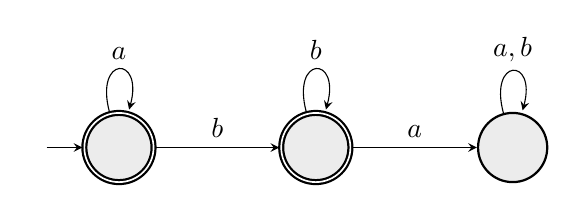
\begin{tikzpicture}
                            \node[state, accepting, initial] (q1) {};
                            \node[state, accepting, right of=q1] (q2) {};
                            \node[state, right of=q2] (q3) {};
                            \draw (q1) edge[loop above] node{$a$} (q1)
                            (q1) edge[above] node{$b$} (q2)
                            (q2) edge[loop above] node{$b$} (q2)
                            (q2) edge[above] node{$a$} (q3)
                            (q3) edge[loop above] node{$a,b$} (q3);
                        \end{tikzpicture}
                        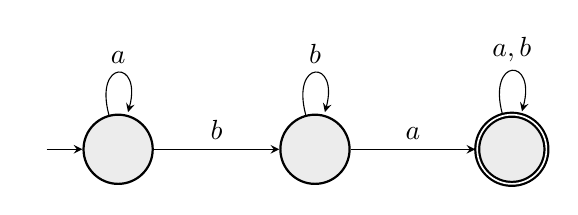
\begin{tikzpicture}
                            \node[state, initial] (q1) {};
                            \node[state, right of=q1] (q2) {};
                            \node[state, accepting, right of=q2] (q3) {};
                            \draw (q1) edge[loop above] node{$a$} (q1)
                            (q1) edge[above] node{$b$} (q2)
                            (q2) edge[loop above] node{$b$} (q2)
                            (q2) edge[above] node{$a$} (q3)
                            (q3) edge[loop above] node{$a,b$} (q3);
                        \end{tikzpicture}
                        \caption{$\overline{F}$ and $F$}
                    \end{figure}
              \item $G= \{w|w~\text{is any string that doesn’t contain exactly two }a\text{’s}\}$

                    $\overline{G} = \{w|w~\text{is any string that contains exactly two }a\text{’s}\}$
                    \begin{figure}[H]
                        \centering
                        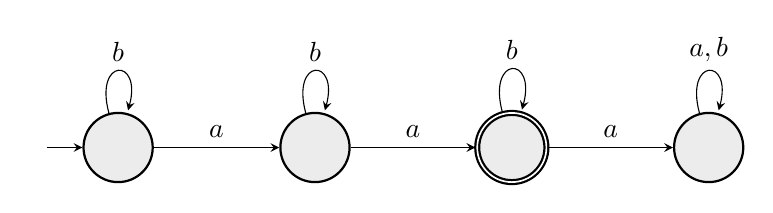
\begin{tikzpicture}
                            \node[state, initial] (q1) {};
                            \node[state, right of=q1] (q2) {};
                            \node[state, accepting, right of=q2] (q3) {};
                            \node[state, right of=q3] (q4) {};
                            \draw (q1) edge[loop above] node{$b$} (q1)
                            (q1) edge[above] node{$a$} (q2)
                            (q2) edge[loop above] node{$b$} (q2)
                            (q2) edge[above] node{$a$} (q3)
                            (q3) edge[loop above] node{$b$} (q3)
                            (q3) edge[above] node{$a$} (q4)
                            (q4) edge[loop above] node{$a,b$} (q4);
                        \end{tikzpicture}
                        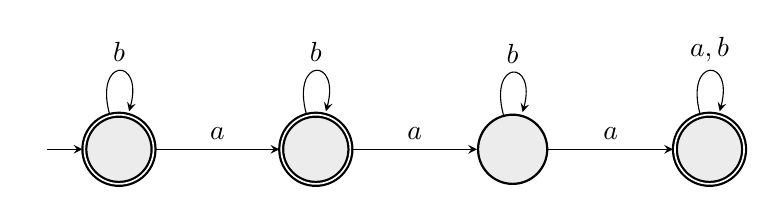
\begin{tikzpicture}
                            \node[state, accepting, initial] (q1) {};
                            \node[state, accepting, right of=q1] (q2) {};
                            \node[state, right of=q2] (q3) {};
                            \node[state, accepting, right of=q3] (q4) {};
                            \draw (q1) edge[loop above] node{$b$} (q1)
                            (q1) edge[above] node{$a$} (q2)
                            (q2) edge[loop above] node{$b$} (q2)
                            (q2) edge[above] node{$a$} (q3)
                            (q3) edge[loop above] node{$b$} (q3)
                            (q3) edge[above] node{$a$} (q4)
                            (q4) edge[loop above] node{$a,b$} (q4);
                        \end{tikzpicture}
                        \caption{$\overline{G}$ and $G$}
                    \end{figure}
              \item $H=\{w|w~\text{is any string except }a\text{ and }b\}$

                    $\overline{H} = \{w|w~\text{is string }a\text{ or }b\}$
                    \begin{figure}[H]
                        \centering
                        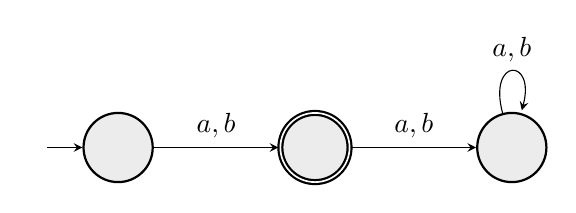
\begin{tikzpicture}
                            \node[state, initial] (q1) {};
                            \node[state, accepting, right of=q1] (q2) {};
                            \node[state, right of=q2] (q3) {};
                            \draw
                            (q1) edge[above] node{$a,b$} (q2)
                            (q2) edge[above] node{$a,b$} (q3)
                            (q3) edge[loop above] node{$a,b$} (q3);
                        \end{tikzpicture}
                        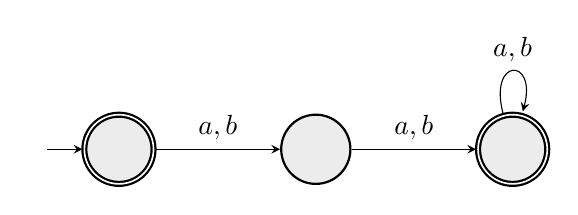
\begin{tikzpicture}
                            \node[state, accepting, initial] (q1) {};
                            \node[state, right of=q1] (q2) {};
                            \node[state, accepting, right of=q2] (q3) {};
                            \draw
                            (q1) edge[above] node{$a,b$} (q2)
                            (q2) edge[above] node{$a,b$} (q3)
                            (q3) edge[loop above] node{$a,b$} (q3);
                        \end{tikzpicture}
                        \caption{$\overline{H}$ and $H$}
                    \end{figure}
          \end{enumerate}

    \item[1.6]
          Give state diagrams of DFAs recognizing the following languages. In all parts,the alphabet is $\{0,1\}$.
          \begin{enumerate}
              \item $\{w|w~ \text{begins with a }1\text{ and ends with a }0\}$
                    \begin{figure}[H]
                        \centering
                        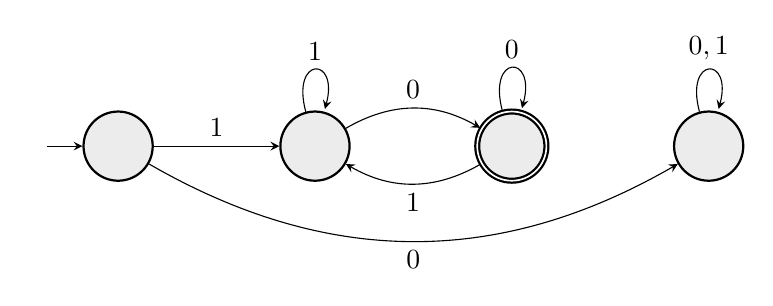
\begin{tikzpicture}
                            \node[state, initial] (q1) {};
                            \node[state, right of=q1] (q2) {};
                            \node[state, accepting, right of=q2] (q3) {};
                            \node[state, right of=q3] (q4) {};
                            \draw
                            (q1) edge[above] node{$1$} (q2)
                            (q2) edge[loop above] node{$1$} (q2)
                            (q2) edge[bend left, above] node{$0$} (q3)
                            (q3) edge[loop above] node{$0$} (q3)
                            (q3) edge[bend left, below] node{$1$} (q2)
                            (q1) edge[bend right, below] node{$0$} (q4)
                            (q4) edge[loop above] node{$0,1$} (q4);
                        \end{tikzpicture}
                    \end{figure}
              \item $\{w|w~ \text{contains at least three }1\text{'s}\}$
                    \begin{figure}[H]
                        \centering
                        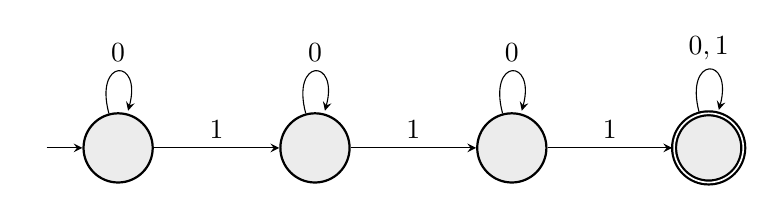
\begin{tikzpicture}
                            \node[state, initial] (q1) {};
                            \node[state, right of=q1] (q2) {};
                            \node[state, right of=q2] (q3) {};
                            \node[state, accepting, right of=q3] (q4) {};
                            \draw
                            (q1) edge[loop above] node{$0$} (q1)
                            (q1) edge[above] node{$1$} (q2)
                            (q2) edge[loop above] node{$0$} (q2)
                            (q2) edge[above] node{$1$} (q3)
                            (q3) edge[loop above] node{$0$} (q3)
                            (q3) edge[above] node{$1$} (q4)
                            (q4) edge[loop above] node{$0,1$} (q4);
                        \end{tikzpicture}
                    \end{figure}
              \item $\{w|w~ \text{contains the substring } 0101~ \text{(i.e., }w = x0101y\text{ for some }x\text{ and }y)\}$
                    \begin{figure}[H]
                        \centering
                        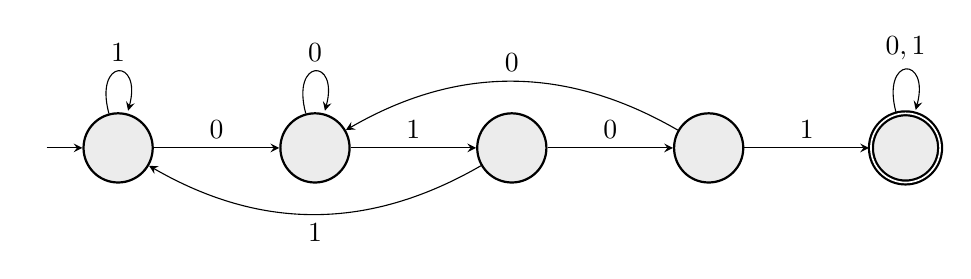
\begin{tikzpicture}
                            \node[state, initial] (q1) {};
                            \node[state, right of=q1] (q2) {};
                            \node[state, right of=q2] (q3) {};
                            \node[state, right of=q3] (q4) {};
                            \node[state, accepting, right of=q4] (q5) {};
                            \draw
                            (q1) edge[loop above] node{$1$} (q1)
                            (q1) edge[above] node{$0$} (q2)
                            (q2) edge[loop above] node{$0$} (q2)
                            (q2) edge[above] node{$1$} (q3)
                            (q3) edge[above] node{$0$} (q4)
                            (q4) edge[above] node{$1$} (q5)
                            (q5) edge[loop above] node{$0,1$} (q5)
                            (q3) edge[bend left, below] node{$1$} (q1)
                            (q4) edge[bend right, above] node{$0$} (q2);
                        \end{tikzpicture}
                    \end{figure}
              \item $\{w|w~ \text{has length at least }3\text{ and its third symbol is a }0\}$
                    \begin{figure}[H]
                        \centering
                        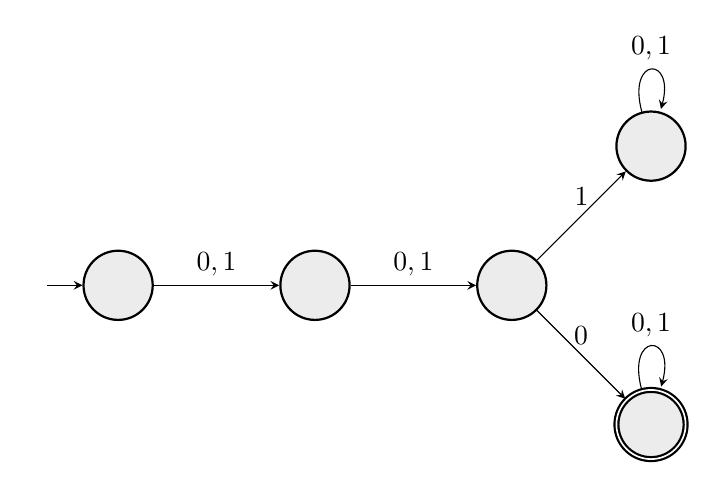
\begin{tikzpicture}
                            \node[state, initial] (q1) {};
                            \node[state, right of=q1] (q2) {};
                            \node[state, right of=q2] (q3) {};
                            \node[state, accepting, below right of=q3] (q4) {};
                            \node[state, above right of=q3] (q5) {};
                            \draw
                            (q1) edge[above] node{$0,1$} (q2)
                            (q2) edge[above] node{$0,1$} (q3)
                            (q3) edge[above] node{$0$} (q4)
                            (q3) edge[above] node{$1$} (q5)
                            (q4) edge[loop above] node{$0,1$} (q4)
                            (q5) edge[loop above] node{$0,1$} (q5);
                        \end{tikzpicture}
                    \end{figure}

              \item $\{w|w~ \text{starts with }0\text{ and has odd length, or starts with }1\text{ and has even length}\}$
                    \begin{figure}[H]
                        \centering
                        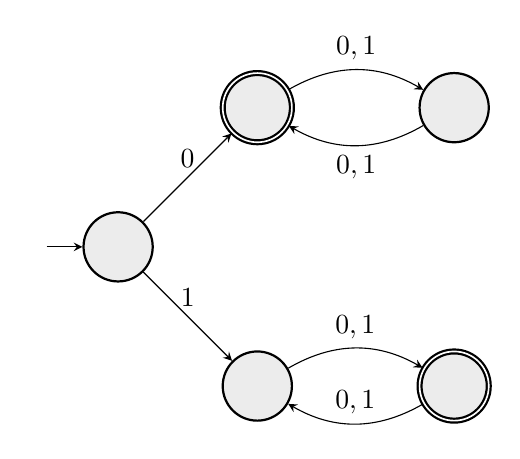
\begin{tikzpicture}
                            \node[state, initial] (q1) {};
                            \node[state, accepting, above right of=q1] (q2) {};
                            \node[state, below right of=q1] (q3) {};
                            \node[state, right of=q2] (q4) {};
                            \node[state, accepting, right of=q3] (q5) {};
                            \draw
                            (q1) edge[above] node{$0$} (q2)
                            (q1) edge[above] node{$1$} (q3)
                            (q2) edge[bend left, above] node{$0,1$} (q4)
                            (q4) edge[bend left, below] node{$0,1$} (q2)
                            (q3) edge[bend left, above] node{$0,1$} (q5)
                            (q5) edge[bend left, above] node{$0,1$} (q3);
                        \end{tikzpicture}
                    \end{figure}
              \item $\{w|w~ \text{doesn't contain the substring }110\}$
                    \begin{figure}[H]
                        \centering
                        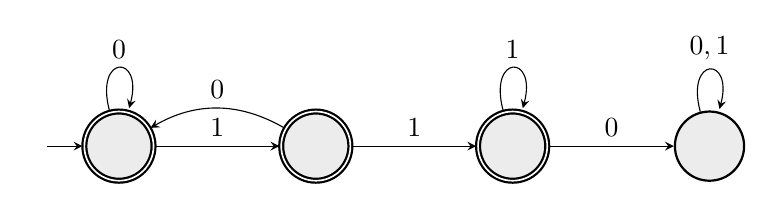
\begin{tikzpicture}
                            \node[state, accepting, initial] (q1) {};
                            \node[state, accepting, right of=q1] (q2) {};
                            \node[state, accepting, right of=q2] (q3) {};
                            \node[state, right of=q3] (q4) {};
                            \draw
                            (q1) edge[above] node{$1$} (q2)
                            (q1) edge[loop above] node{$0$} (q1)
                            (q2) edge[above] node{$1$} (q3)
                            (q2) edge[bend right, above] node{$0$} (q1)
                            (q3) edge[above] node{$0$} (q4)
                            (q3) edge[loop above] node{$1$} (q3)
                            (q4) edge[loop above] node{$0,1$} (q4);
                        \end{tikzpicture}
                    \end{figure}
              \item $\{w|\text{the length of }w\text{ is at most }5\}$

                    \begin{figure}[H]
                        \centering
                        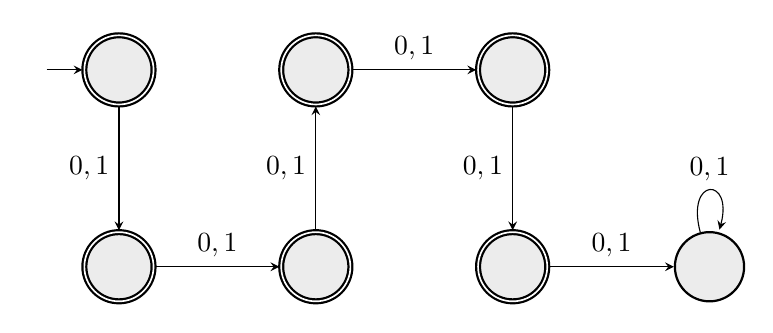
\begin{tikzpicture}
                            \node[state, accepting, initial] (q1) {};
                            \node[state, accepting, below of=q1] (q2) {};
                            \node[state, accepting, right of=q2] (q3) {};
                            \node[state, accepting, above of=q3] (q4) {};
                            \node[state, accepting, right of=q4] (q5) {};
                            \node[state, accepting, below of=q5] (q6) {};
                            \node[state, right of=q6] (q7) {};
                            \draw
                            (q7) edge[loop above] node{$0,1$} (q7)
                            (q1) edge[left] node{$0,1$} (q2)
                            (q2) edge[above] node{$0,1$} (q3)
                            (q3) edge[left] node{$0,1$} (q4)
                            (q4) edge[above] node{$0,1$} (q5)
                            (q5) edge[left] node{$0,1$} (q6)
                            (q6) edge[above] node{$0,1$} (q7);
                        \end{tikzpicture}
                    \end{figure}

              \item $\{w|w~ \text{is any string except }11\text{ and }111\}$
                    \begin{figure}[H]
                        \centering
                        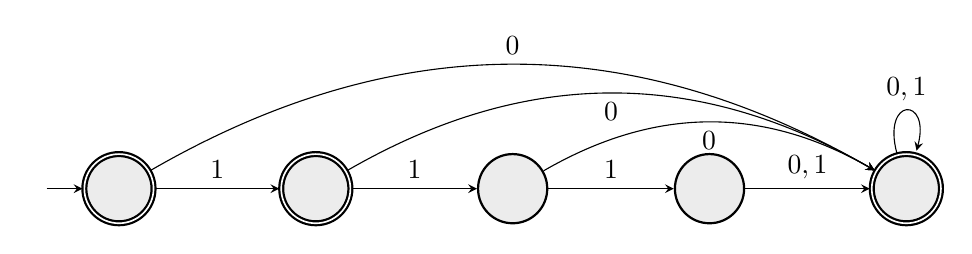
\begin{tikzpicture}
                            \node[state, accepting, initial] (q1) {};
                            \node[state, accepting, right of=q1] (q2) {};
                            \node[state, right of=q2] (q3) {};
                            \node[state, right of=q3] (q4) {};
                            \node[state, accepting, right of=q4] (q5) {};
                            \draw
                            (q1) edge[above] node{$1$} (q2)
                            (q1) edge[bend left, above] node{$0$} (q5)
                            (q2) edge[above] node{$1$} (q3)
                            (q2) edge[bend left, below ] node{$0$} (q5)
                            (q3) edge[above] node{$1$} (q4)
                            (q3) edge[bend left, below] node{$0$} (q5)
                            (q4) edge[above] node{$0,1$} (q5)
                            (q5) edge[loop above] node{$0,1$} (q5);
                        \end{tikzpicture}
                    \end{figure}
              \item $\{w|\text{ every odd position of }w\text{ is a }1\}$
                    \begin{figure}[H]
                        \centering
                        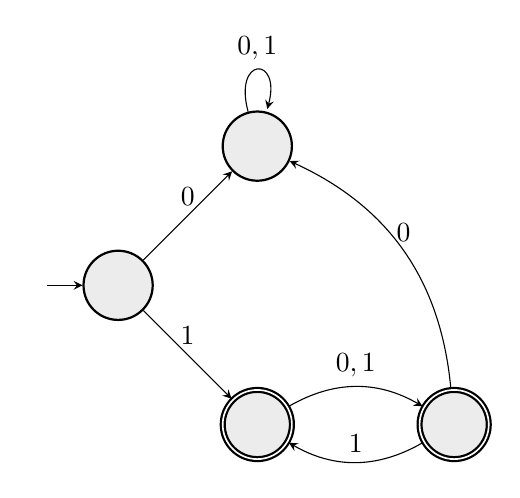
\begin{tikzpicture}
                            \node[state, initial] (q1) {};
                            \node[state, above right of=q1] (q2) {};
                            \node[state, accepting, below right of=q1] (q3) {};
                            \node[state, accepting, right of=q3] (q5) {};
                            \draw
                            (q1) edge[above] node{$0$} (q2)
                            (q1) edge[above] node{$1$} (q3)
                            (q2) edge[loop above] node{$0,1$} (q2)
                            (q3) edge[bend left, above] node{$0,1$} (q5)
                            (q5) edge[bend left, above] node{$1$} (q3)
                            (q5) edge[bend right, above] node{$0$} (q2);
                        \end{tikzpicture}
                    \end{figure}
              \item $\{w|w~ \text{contains at least two }0\text{'s and at most one }1\}$
                    \begin{figure}[H]
                        \centering
                        \begin{tikzpicture}
                            \node[state, initial] (q1) {};
                            \node[state, above right of=q1] (q2) {};
                            \node[state, below right of=q1] (q3) {};
                            \node[state, below right of=q2] (q4) {};
                            \node[state, accepting, above right of=q2] (q5) {};
                            \node[state, below right of=q3] (q8) {};
                            \node[state, accepting, right of=q4] (q6) {};
                            \draw
                            (q1) edge[above] node{$0$} (q2)
                            (q1) edge[above] node{$1$} (q3)
                            (q2) edge[above] node{$0$} (q5)
                            (q2) edge[above] node{$1$} (q4)
                            (q3) edge[above] node{$0$} (q4)
                            (q3) edge[above] node{$1$} (q8)
                            (q4) edge[above] node{$0$} (q6)
                            (q4) edge[right] node{$1$} (q8)
                            (q5) edge[above] node{$1$} (q6)
                            (q5) edge[loop right] node{$0$} (q5)
                            (q6) edge[loop above] node{$0$} (q6)
                            (q8) edge[loop right] node{$0,1$} (q8)
                            (q6) edge[above] node{$1$} (q8);
                        \end{tikzpicture}
                    \end{figure}
              \item $\{\epsilon,0\}$
                    \begin{figure}[H]
                        \centering
                        \begin{tikzpicture}
                            \node[state, initial, accepting] (q1) {};
                            \node[state, accepting, above right of=q1] (q2) {};
                            \node[state, below right of=q1] (q3) {};
                            \draw
                            (q1) edge[above] node{$0$} (q2)
                            (q1) edge[right] node{$1$} (q3)
                            (q2) edge[right] node{$0,1$} (q3)
                            (q3) edge[loop right] node{$0,1$} (q3);
                        \end{tikzpicture}
                    \end{figure}
              \item $\{w|w~ \text{contains an even number of }0\text{'s, or contains exactly two }1\text{'s}\}$
                    \begin{figure}[H]
                        \centering
                        \begin{tikzpicture}
                            \node[state, initial, accepting] (q1) {};
                            \node[state, accepting, above right of=q1] (q2) {};
                            \node[state, below right of=q1] (q3) {};
                            \node[state, accepting, right of=q3] (q4) {};
                            \node[state, right of=q2] (q5) {};
                            \node[state, accepting, above right of=q2] (q6) {};
                            \node[state, accepting, right of=q6] (q7) {};
                            \node[state, accepting, above right of=q6] (q8) {};
                            \node[state, right of=q8] (q9) {};
                            \draw
                            (q1) edge[above] node{$1$} (q2)
                            (q1) edge[right] node{$0$} (q3)
                            (q3) edge[below] node{$1$} (q5)
                            (q4) edge[bend right, below] node{$1$} (q2)
                            (q3) edge[bend right, above] node{$0$} (q4)
                            (q4) edge[bend right, below] node{$0$} (q3)
                            (q2) edge[bend right, above] node{$0$} (q5)
                            (q2) edge[right, above] node{$1$} (q6)
                            (q5) edge[right, below] node{$1$} (q7)
                            (q5) edge[bend right, below] node{$0$} (q2)
                            (q6) edge[bend right, above] node{$0$} (q7)
                            (q7) edge[bend right, below] node{$0$} (q6)
                            (q6) edge[right, above] node{$1$} (q8)
                            (q7) edge[right, below] node{$1$} (q9)
                            (q8) edge[bend right, above] node{$0$} (q9)
                            (q9) edge[bend right, below] node{$0$} (q8);
                        \end{tikzpicture}
                    \end{figure}
              \item The empty set
                    \begin{figure}[H]
                        \centering
                        \begin{tikzpicture}
                            \node[state, initial] (q1) {};
                            \draw
                            (q1) edge[loop right] node{$0,1$} (q1);
                        \end{tikzpicture}
                    \end{figure}
              \item All strings except the empty string
                    \begin{figure}[H]
                        \centering
                        \begin{tikzpicture}
                            \node[state, initial] (q1) {};
                            \node[state, accepting, right of=q1] (q2) {};
                            \draw
                            (q1) edge[above] node{$0,1$} (q2)
                            (q2) edge[loop above] node{$0,1$} (q2);
                        \end{tikzpicture}
                    \end{figure}
          \end{enumerate}
\end{enumerate}

\include{chapter01-exercises-107-112}
\include{chapter01-exercises-113-117}
\end{document}
